\chapter{Analisis}
\label{chap:analisis}

Pada bab ini akan dijelaskan mengenai analisis pemanfaatan jsoup untuk mengambil data mahasiswa, dan analisis pemanfaatan JavaFX untuk membuat tampilan antarmuka pengguna.

\section{Analisis Pemanfaatan Jsoup}
Untuk mengambil data mahasiswa, diperlukan sumber data mahasiswa tersebut. Sumber data mahasiswa tersebut dapat diperoleh melalui Portal Akademik Mahasiswa. Portal Akademik Mahasiswa merupakan sebuah situs yang diperuntukkan bagi mahasiswa untuk mendapatkan informasi mengenai profil dan kegiatan akademik mahasiswa tersebut. Mahasiswa dapat mengakses Portal Akademik Mahasiswa melalui \textit{URL} \url{https://studentportal.unpar.ac.id/}. Untuk mengakses Portal Akademik Mahasiswa, mahasiswa harus melakukan \textit{login} menggunakan \textit{email} dan \textit{password} mahasiswa tersebut.

Pada halaman utama Portal Akademik Mahasiswa (Gambar \ref{fig:3_home}), terdapat beberapa menu yang dapat digunakan sebagai sumber data yaitu:

\begin{figure}[H]
	\centering
	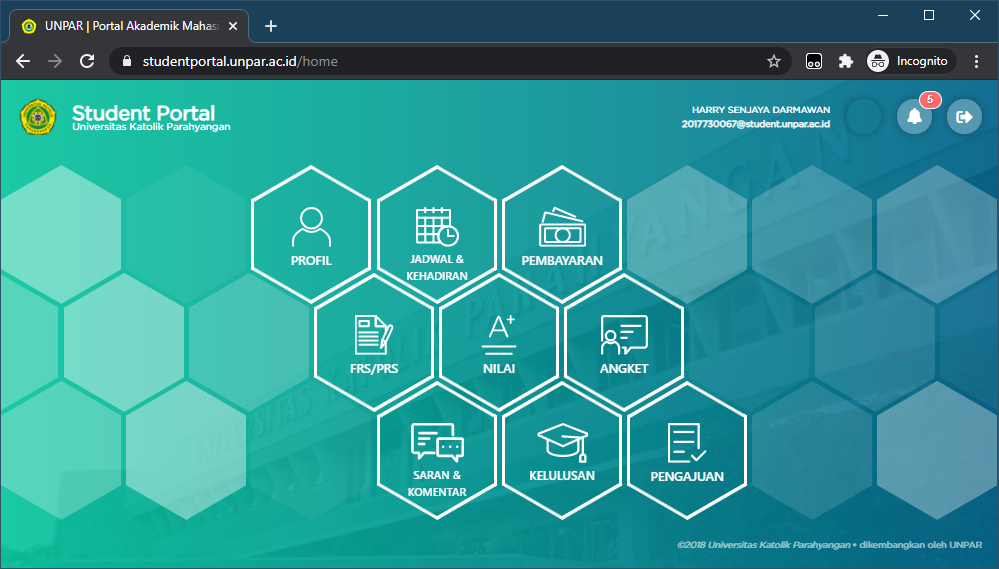
\includegraphics[scale=0.45]{Gambar/home.png}
	\caption{Halaman Utama Portal Akademik Mahasiswa} 
	\label{fig:3_home}
\end{figure}

\begin{enumerate}
    \item \textbf{Profil}, merupakan halaman yang menampilkan data diri mahasiswa (Gambar \ref{fig:3_profil}).
    
    \begin{figure}[H]
    	\centering
    	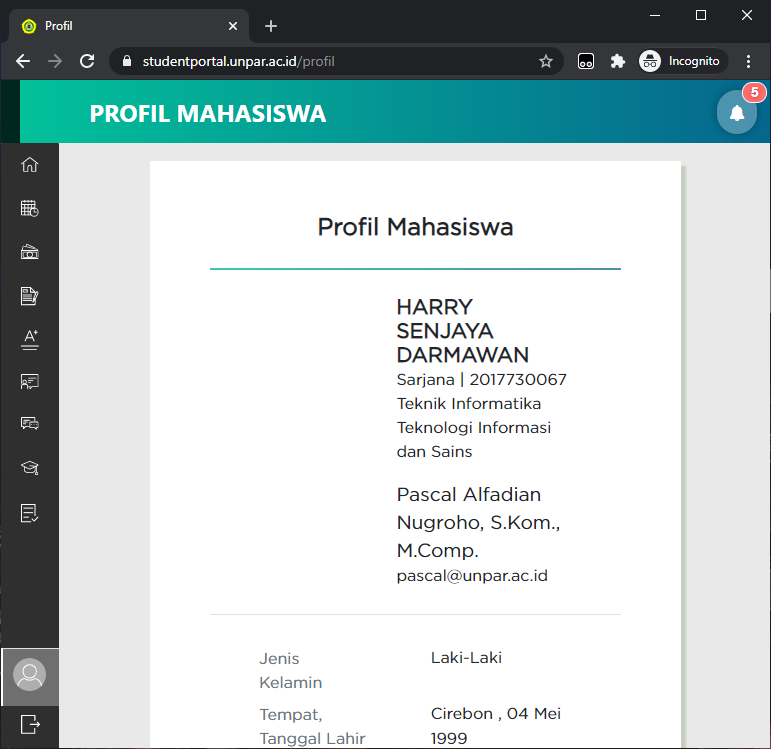
\includegraphics[scale=0.45]{Gambar/profil.png}
    	\caption{Halaman Profil} 
    	\label{fig:3_profil}
    \end{figure}
    
    \item \textbf{Nilai}, terdiri dari beberapa submenu:
    
    \begin{itemize}
        \item Nilai per Semester\\
        Submenu ini menampilkan informasi nilai per semester. Mahasiswa dapat melihat nilai sesuai dengan semester yang dipilih (Gambar \ref{fig:3_nilai_per_semester}).
        
        \begin{figure}[H]
        	\centering
        	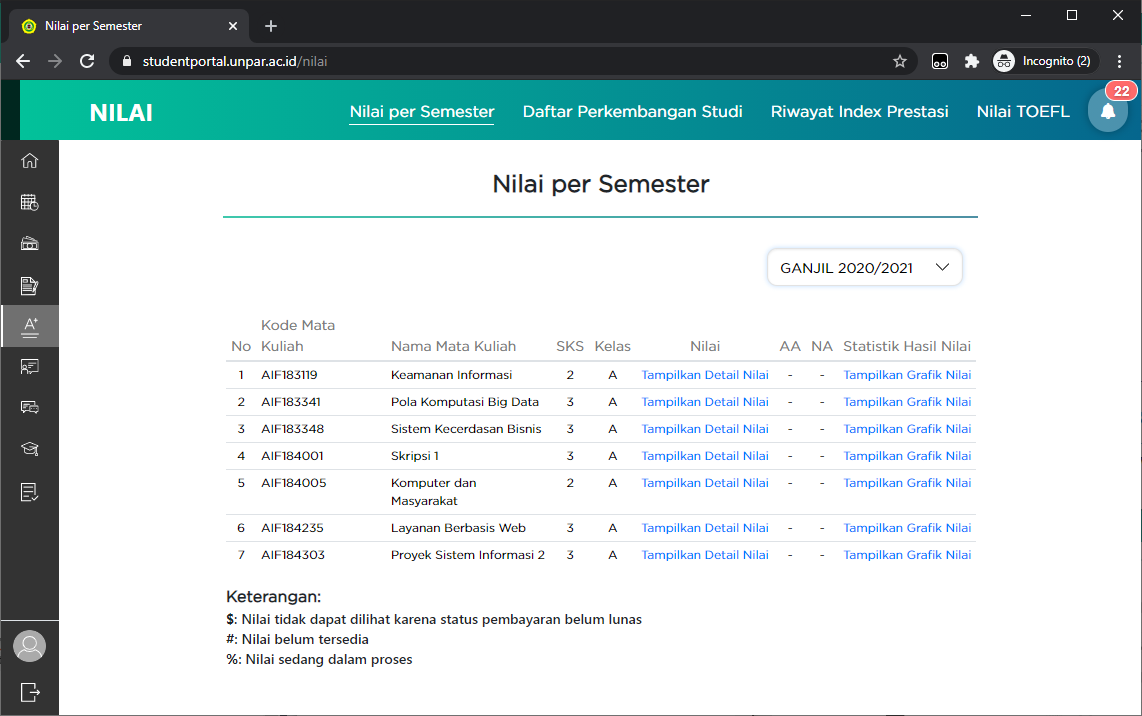
\includegraphics[scale=0.4]{Gambar/nilai_per_semester.png}
        	\caption{Halaman Nilai Per Semester} 
        	\label{fig:3_nilai_per_semester}
        \end{figure}
        
        \item Daftar Perkembangan Studi\\
       Submenu ini menampilkan seluruh riwayat mata kuliah dan nilai yang pernah ditempuh mahasiswa (Gambar \ref{fig:3_dps_1}). Submenu ini juga menampilkan statistik sks, nilai, dan indeks prestasi mahasiswa (Gambar \ref{fig:3_dps_2}).
        
        \begin{figure}[H]
        	\centering
        	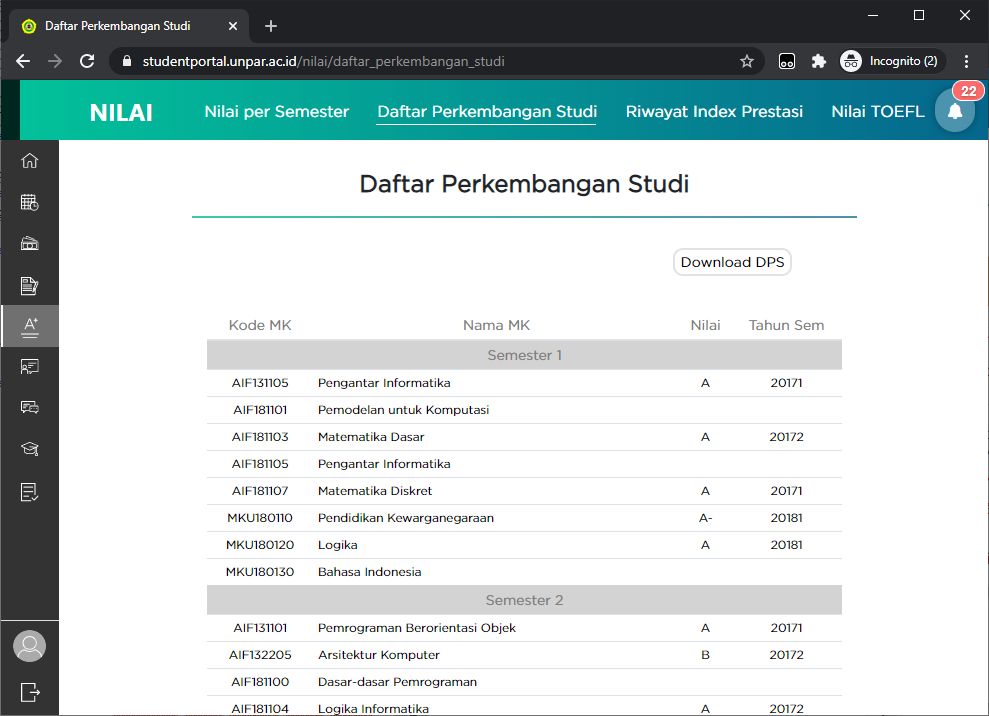
\includegraphics[scale=0.4]{Gambar/nilai_dps_1.png}
        	\caption{Halaman Daftar Perkembangan Studi (1)} 
        	\label{fig:3_dps_1}
        \end{figure}
        
         \begin{figure}[H]
        	\centering
        	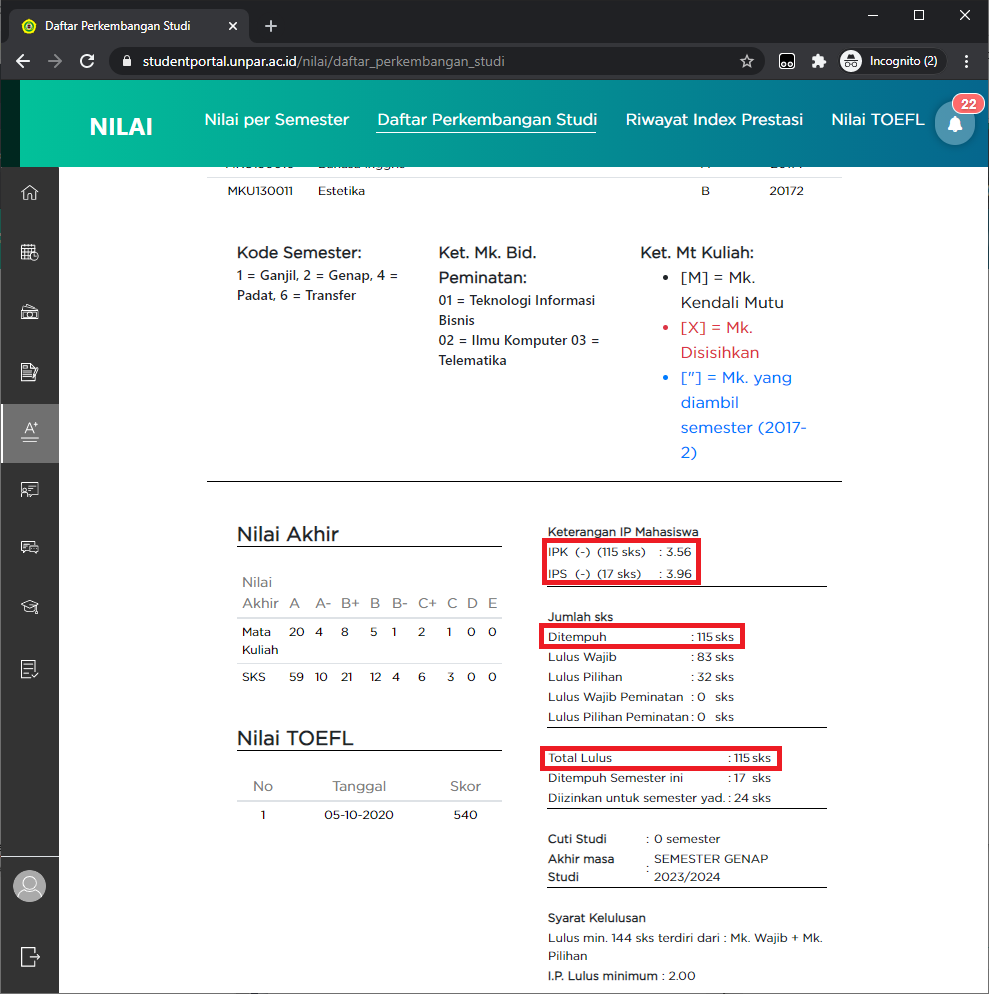
\includegraphics[scale=0.4]{Gambar/nilai_dps_2.png}
        	\caption{Halaman Daftar Perkembangan Studi (2)} 
        	\label{fig:3_dps_2}
        \end{figure}
        
        \item Riwayat Indeks Prestasi\\
       Submenu ini menampilkan seluruh riwayat Indeks Prestasi Semester (IPS) dan Indeks Prestasi Kumulatif (IPK) setiap semester mahasiswa (Gambar \ref{fig:3_rip}).
       
       \begin{figure}[H]
        	\centering
        	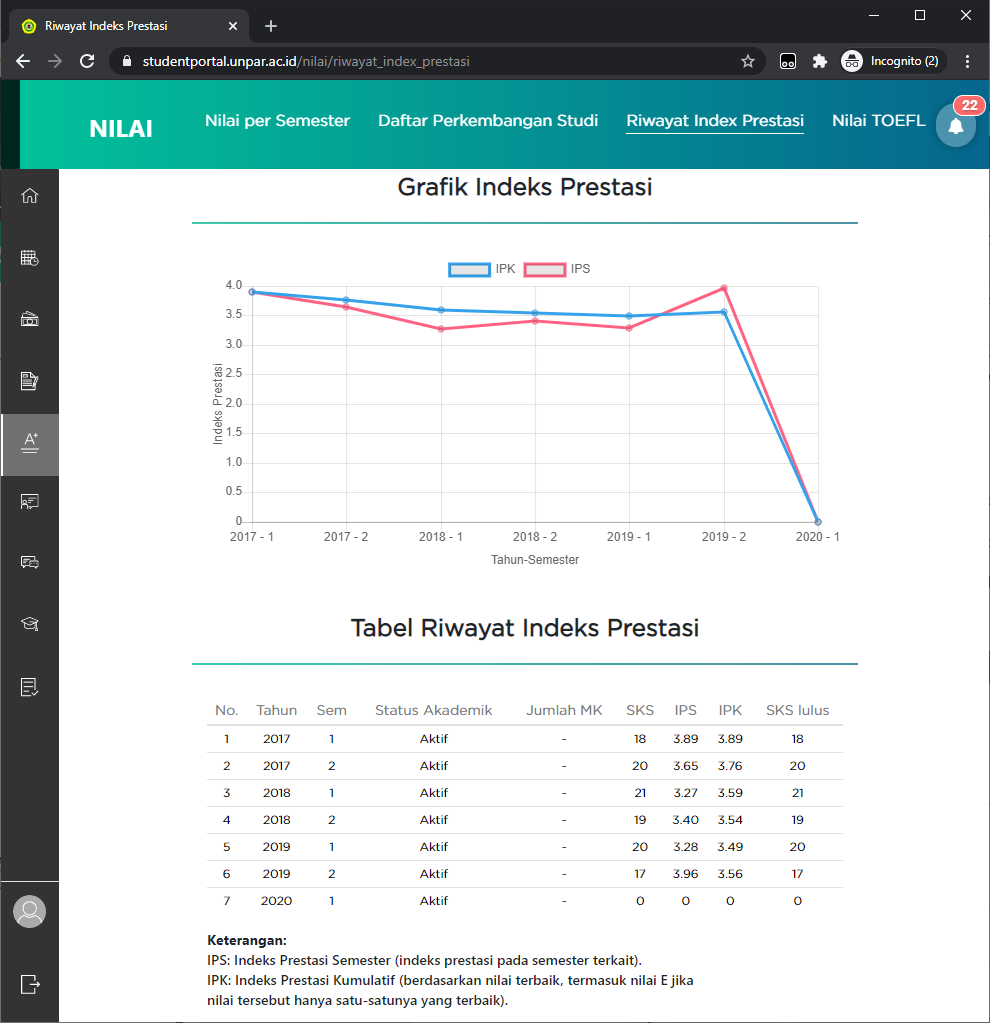
\includegraphics[scale=0.4]{Gambar/nilai_rip.png}
        	\caption{Halaman Riwayat Indeks Prestasi} 
        	\label{fig:3_rip}
        \end{figure}
        
        \item Nilai TOEFL\\
       Submenu ini menampilkan seluruh riwayat skor dan detail skor \textit{Test of English as Foreign Language} (TOEFL) yang pernah ditempuh mahasiswa (Gambar \ref{fig:3_toefl}).
       
       \begin{figure}[H]
        	\centering
        	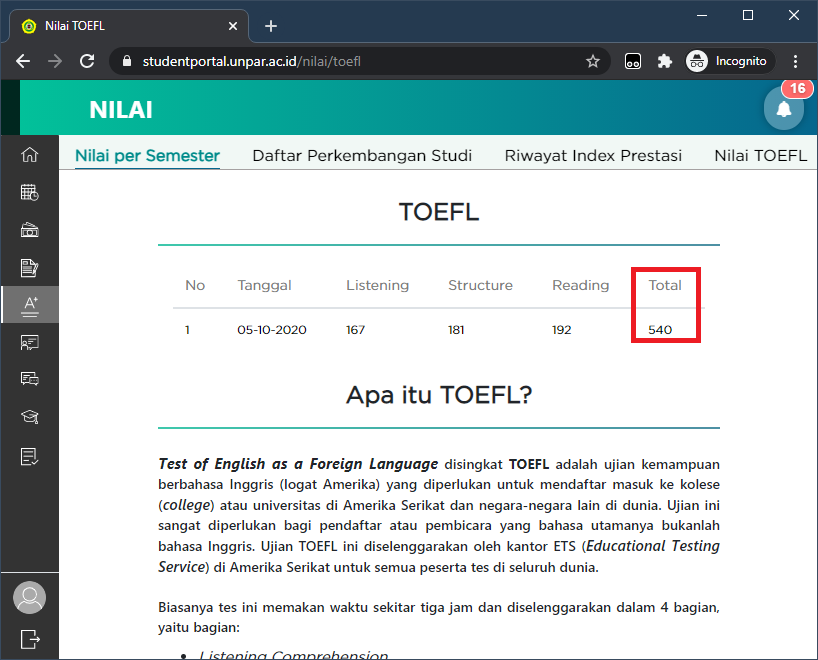
\includegraphics[scale=0.4]{Gambar/nilai_toefl.png}
        	\caption{Halaman Nilai TOEFL} 
        	\label{fig:3_toefl}
        \end{figure}
    \end{itemize}
\end{enumerate}

Aplikasi \textit{screen saver} akan melakukan \textit{http} ke Student Portal UNPAR untuk mendapatkan data untuk setiap kebutuhan dari masing-masing fitur yang ada. Pengambilan data secara langsung dari Student Portal UNPAR dilakukan menggunakan \textit{library} jsoup. Pemanfaatan jsoup untuk mengambil data-data tersebut sudah diimplementasikan pada skripsi Andrianto Sugiarto \cite{ifstupor} sebelumnya. Data yang telah didapat dari Student Portal UNPAR kemudian diolah ke dalam SIAModels, dan ditampilkan sesuai dengan fitur-fitur yang ada pada aplikasi Mahasiswa Wali \textit{Screen Saver}.

